\chapter{Finite Element Modeling}
\label{chap:FEM}

This chapter outlines the development of the finite element model of the UBX metro and the simulation setup. First, in section \ref{section:geometry}, the design of the model geometry and the mesh of the model are shown. Consecutively, section \ref{section:boundary_conditions} describes the incorporation of boundary conditions into the finite element model. Finally, in section \ref{section:parametric_study}, a parametric study is carried out to investigate the influence of different simulation parameters on the solution of the initial finite element model. All these simulations are executed with the acoustics module of the open-source FEM software openCFS \cite{opencfs}.


\section{Geometry and mesh}
\label{section:geometry}

Due to the large dimension of the car body, the computation of the complete model would be too extensive. Hence, the simulation model constitutes of the front bogie part only. The latter has been marked through a red box in fig. \ref{fig:red_box}. Furthermore, the outer pressure field measurement described in sec. \ref{sec:pressure_field_measurement} has been taken from the same area.


\begin{figure}[H]
	\centering
	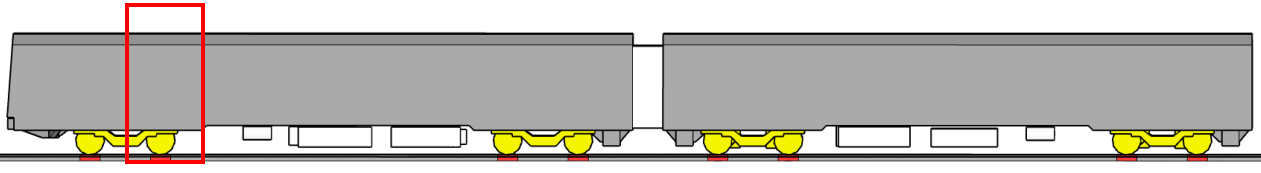
\includegraphics[width=\textwidth]{fig/chap4/geometry/model_area.png}
	\caption{Side view of UBX, red box indicates the modeling area}
	\label{fig:red_box}
\end{figure}

In order to reduce computational effort, the symmetry of the model is exploited. The quarter model is depicted in fig. \ref{fig:fourth_model}, whereas the equivalent model, namely the full model, is shown in fig. \ref{fig:full_model}. Both models are shown for more comprehensive illustration of the modeled underfloor components, but only the quarter model has been used in the simulation. For simplification of the geometry design, exclusively the most essential components have been included in the model. Starting with the squared car body (dark green), the bogie (purple), the wheel (pink), the air suspension (gray) and ending with the omnidirectional loudspeaker (bright green). This respective component has been placed underneath the car floor, between bogie and the wheel axle and is represented through a sphere with $35\,\text{cm}$ diameter.


\begin{figure}[H]
	\centering
	\begin{subfigure}[b]{0.4\textwidth}
		\centering
		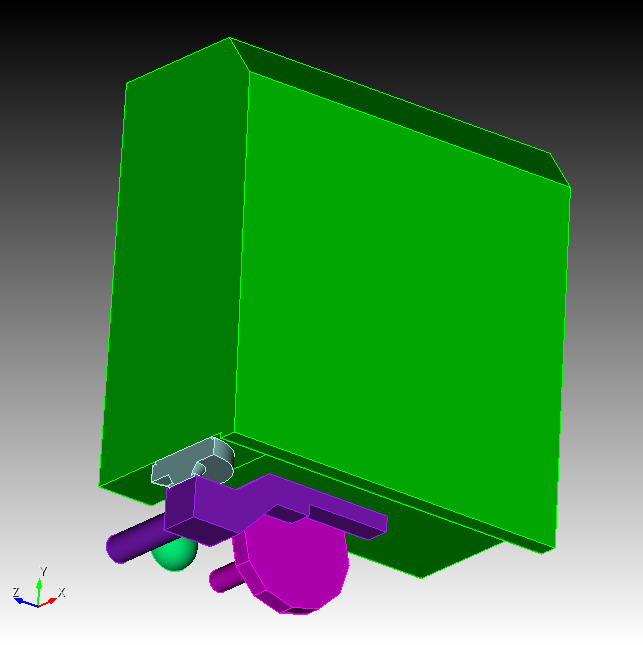
\includegraphics[width=0.9\linewidth]{fig/chap4/geometry/one_fourth_model.png}
		\caption{quarter model}
		\label{fig:fourth_model}
	\end{subfigure}
	\hfill
	\begin{subfigure}[b]{0.4\textwidth}
		\centering
		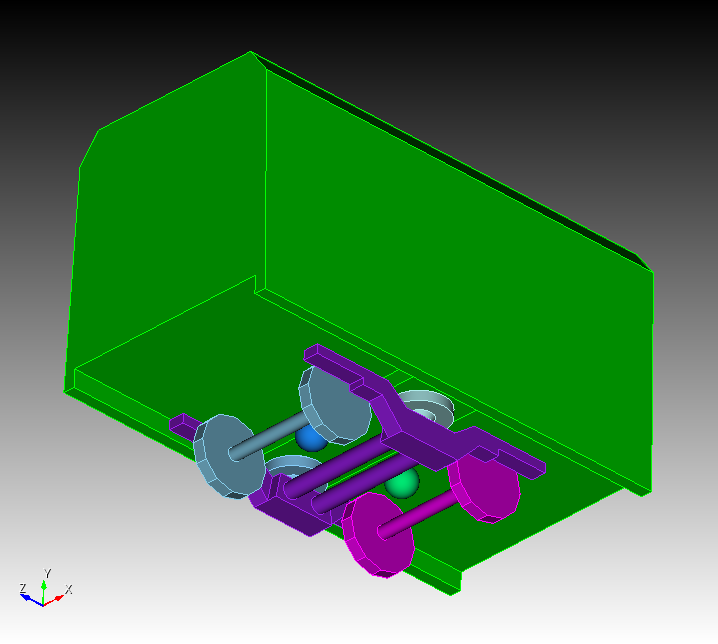
\includegraphics[width=\linewidth]{fig/chap4/geometry/initial_model_2.png}
		\caption{full model}
		\label{fig:full_model}
	\end{subfigure}
	\caption{Geometry of model}
\end{figure}

The quarter model has been cut out from an acoustic region, surrounded by a perfectly matched layer to simulate the free field condition.

is surrounded by pml to model the open infinite domain

A mesh has been created from the 3d model.

\begin{figure}[H]
	\centering
	\begin{subfigure}[b]{0.45\textwidth}
		\centering
		\includegraphics[width=\linewidth]{fig/chap4/mesh/propagation_domain.png}
		\caption{Propagation region (green) surrounded by a PML (gray)}
		\label{fig:propagation_domain}
	\end{subfigure}
	\hfill
	\begin{subfigure}[b]{0.45\textwidth}
		\centering
		\includegraphics[width=\linewidth]{fig/chap4/mesh/mesh1.png}
		\caption{mesh of the acoustic region}
		\label{fig:mesh_model}
	\end{subfigure}
	\caption{Acoustic region}
\end{figure}




\subsection*{Determination of simulation domain}

The goal of this section is to find an appropriate propagation domain size to achieve sufficient numerical accuracy while keeping the computational effort low. For the variation, the length and height of the propagation domain are kept constant while only the width of the domain is varied.

\begin{figure}[H]
	\centering
	\begin{subfigure}[b]{0.45\textwidth}
		\centering
		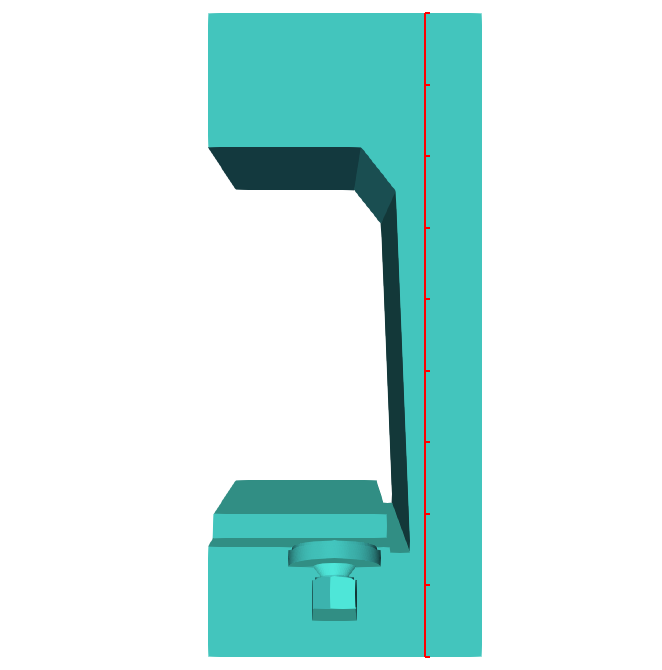
\includegraphics[width=\linewidth]{fig/chap4/simulation_domain/0pt5m.png}
		\caption{0.5 m}
	\end{subfigure}
	\hfill
	\begin{subfigure}[b]{0.45\textwidth}
		\centering
		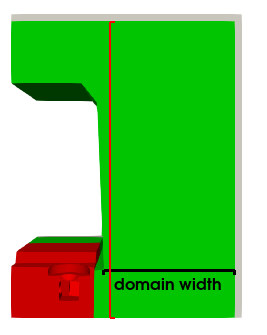
\includegraphics[width=\linewidth]{fig/chap4/simulation_domain/2m.png}
		\caption{2 m}
	\end{subfigure}
	\caption{Models with different simulation domain size}
	\label{fig:domain_size_variation}
\end{figure}

The compared simulation domain size are 0.2 m, 0.5 m, 1 m, 1.5 m and 2m. For each setup, the pressure is evaluated at 0.1 m away from the vehicle along the height direction, and the result is compared to a , the model with 2 m domain size will be used as reference. Fig. \ref{fig:domain_size_variation} shows the model with 0.5 m domain size and the reference model with 2 m domain size. The evaluation position is marked by the red line.

A fictitious excitation with uniform normal surface particle velocity of $u_s = 1\,mm/s$ is applied to the loudspeaker surface.

The reference solution is computed by using a model with 2 m width and all errors are evaluated with respect to this reference.



\subsection*{Computational Effort}
The aim of this section is 

\begin{table}[H]
	\caption{Computational effort for different 1/3-octave frequency band}
	\begin{tabularx}{\textwidth}{|X|X|c|X|X|X|}
		\hline
		1/3-octave center frequency (Hz) & Lower/upper frequency (Hz) & Mesh used                       & Degree of freedoms            & Memory requirement (GB) & Solve time per 9 harmonic steps (hour) \\ \hline
		100                              & 89/112                     & \multirow{10}{*}{1000 Hz 1.5 m} & \multirow{10}{*}{0.8 Million} & \multirow{10}{*}{20}    & \multirow{10}{*}{0.5}                  \\ \cline{1-2}
		125                              & 112/141                    &                                 &                               &                         &                                        \\ \cline{1-2}
		160                              & 141/178                    &                                 &                               &                         &                                        \\ \cline{1-2}
		200                              & 178/224                    &                                 &                               &                         &                                        \\ \cline{1-2}
		250                              & 224/283                    &                                 &                               &                         &                                        \\ \cline{1-2}
		315                              & 283/356                    &                                 &                               &                         &                                        \\ \cline{1-2}
		400                              & 356/449                    &                                 &                               &                         &                                        \\ \cline{1-2}
		500                              & 449/565                    &                                 &                               &                         &                                        \\ \cline{1-2}
		630                              & 565/713                    &                                 &                               &                         &                                        \\ \cline{1-2}
		800                              & 713/897                    &                                 &                               &                         &                                        \\ \hline
		1000                             & 897/1131                   & \multirow{2}{*}{1600 Hz 1 m}    & \multirow{2}{*}{2.3 Million}  & \multirow{2}{*}{70}     & \multirow{2}{*}{2}                     \\ \cline{1-2}
		1250                             & 1131/1425                  &                                 &                               &                         &                                        \\ \hline
		1600                             & 1425/1796                  & 2000 Hz 1 m                     & 4.4 Million                   & 150                     & 5.5                                    \\ \hline
		2000                             & 1796/2262                  & 2300 Hz 1 m                     & 6.6 Million                   & 260                     & 12                                     \\ \hline
	\end{tabularx}
\end{table}


\section{Boundary conditions and loads}
\label{section:boundary_conditions}

After the considerations of the geometrical model, the physical modeling aspects will be discussed. The dominating boundary condition in the finite element model of UBX is the Neumann type boundary condition, which specifies the acoustic particle velocity at the boundary.

The concrete ground $\Gamma_{\text{ground}}$ and the wrapped surfaces of the vehicle components $\Gamma_{\text{vehicle}}$ are assumed to be fully reflective. This also applies to the both symmetry planes (X-Y and Z-Y plane) of the quarter air domain $\Gamma_{\text{symmetry}}$. Hence, the sound hard boundary condition is used for these surfaces

\begin{equation}
	\nabla p \cdot \vec{n} = 0\qquad\text{on}\qquad\Gamma_{\text{ground}}\,\cup\,\Gamma_{\text{vehicle}}\,\cup\,\Gamma_{\text{symmetry}}\text{.}
\end{equation}


To model the infinite domain, the three open surfaces of the propagation domain are surrounded by perfectly matched layers.


A familiar example of a normal velocity boundary is a vibrating mechanical structure that produces sound waves into the surrounding medium



\begin{table}[H]
	\centering
	\caption{Material properties used for the simulation}
	\begin{tabular}{|c|c|}
		\hline
		\textbf{Properties} & \textbf{Value}                   \\ \hline
		Density             &  $1.205\,\text{kg}\cdot \text{m}^{-3}$                     \\ \hline
		Bulk modulus        &  $1.41767\cdot10^5\,\text{Pa}$ \\ \hline
	\end{tabular}
\end{table}

\subsection*{Modeling of sound source}

The loudspeaker sound source is modeled as a pulsating sphere radiating into free field, which is excited by a prescribed surface normal velocity $\hat{u}(a)$ at source radius $a$.

The pressure amplitude of a spherical wave at radius $r$ from the source is given by
\begin{equation}
	\hat{p}(r) = \frac{A}{r}\cdot e^{-jkr}\text{,}
\end{equation}
with $A$ being the monopole amplitude and $k$ being the wave number of the propagating wave.

The relationship between the pressure amplitude and the amplitude of particle velocity is described by the specific acoustic impedance, which is given by
\begin{equation}
	z(r) = \frac{\hat{p}(r)}{\hat{u}(r)} = \rho_0 c_0\frac{jkr}{1+jkr}\text{,} \label{eq:specific_impedance}
\end{equation}
where $\rho_0$ the density of the propagation medium and $c_0$ the speed of sound in the medium. The product $\rho_0 c_0 = z_0$ is also called the characteristic impedance of the propagation medium. (\ref{eq:specific_impedance}) shows that for spherical wave, the acoustic pressure and the particle velocity are not in phase. For very small distances or low frequencies, phases differ by nearly $90^{\circ}$ and in the acoustic far field ($kr >> 1$), the spherical wave can be approximated by plane wave propagation.

For stationary sound field, the average power density or sound intensity is given by
\begin{align}
	\bar{I}(r) &= \frac{1}{2}\text{Re}\lbrace\hat{p}(r)\hat{u}^*(r)\rbrace \\
	&=\frac{1}{2}\frac{|A|^2}{r^2z_0}\qquad \text{.}
\end{align}

The acoustic power of a steady sound source radiating into free field is obtained by integrating the sound intensity over a surface, which encloses the sound source and can be found as
\begin{align}
	W &= \oint_{\Gamma} \bar{I}(r) d\Gamma \\
	  &= \bar{I}(r)\cdot 4\pi r^2 \\
	  &= \frac{2\pi |A|^2}{z_0} \qquad \text{.} \label{eq:acoustic_power}
\end{align}

As apparent in (\ref{eq:acoustic_power}), the acoustic power is independent from the distance to the source.

With the goal of assessing the acoustic power $W$, an expression for the monopole amplitude $A$ has to be determined and inserted into (\ref{eq:acoustic_power}). On the surface of the source, the pressure is given by the product of the surface normal velocity $\hat{u}(a)$ and the specific impedance $z(a)$ evaluated at the source radius and is found by
\begin{equation}
	\hat{p}(a) = \frac{A}{a}\cdot e^{-jka} = \hat{u}(a)\cdot z(a) \qquad \text{.}
\end{equation}

Upon bringing the monopole amplitude $A$ to one side of the equation
\begin{equation}
	A = a\cdot\hat{u}(a)\cdot z(a)\cdot e^{jka}\qquad\text{,}
\end{equation}

and inserting into (\ref{eq:acoustic_power}), the acoustic power can hence be expressed by the surface normal velocity

\begin{equation}
	W = 2\pi a^2\cdot|\hat{u}(a)|^2\cdot z_0 \cdot \frac{(ka)^2}{1+(ka)^2} \qquad\text{.}
\end{equation}

After solving for $|\hat{u}(a)|$

\begin{equation}
	|\hat{u}(a)| = \sqrt{\frac{W\cdot(1 + k^2a^2)}{2\pi z_0 k^2a^4}} \label{eq:input_velocity}
\end{equation}

the relationship between input surface normal velocity and the output acoustic power has been established. Through (\ref{eq:input_velocity}), the required surface normal velocity for a given source acoustic power can be calculated.

\begin{figure}[H]
	\centering
	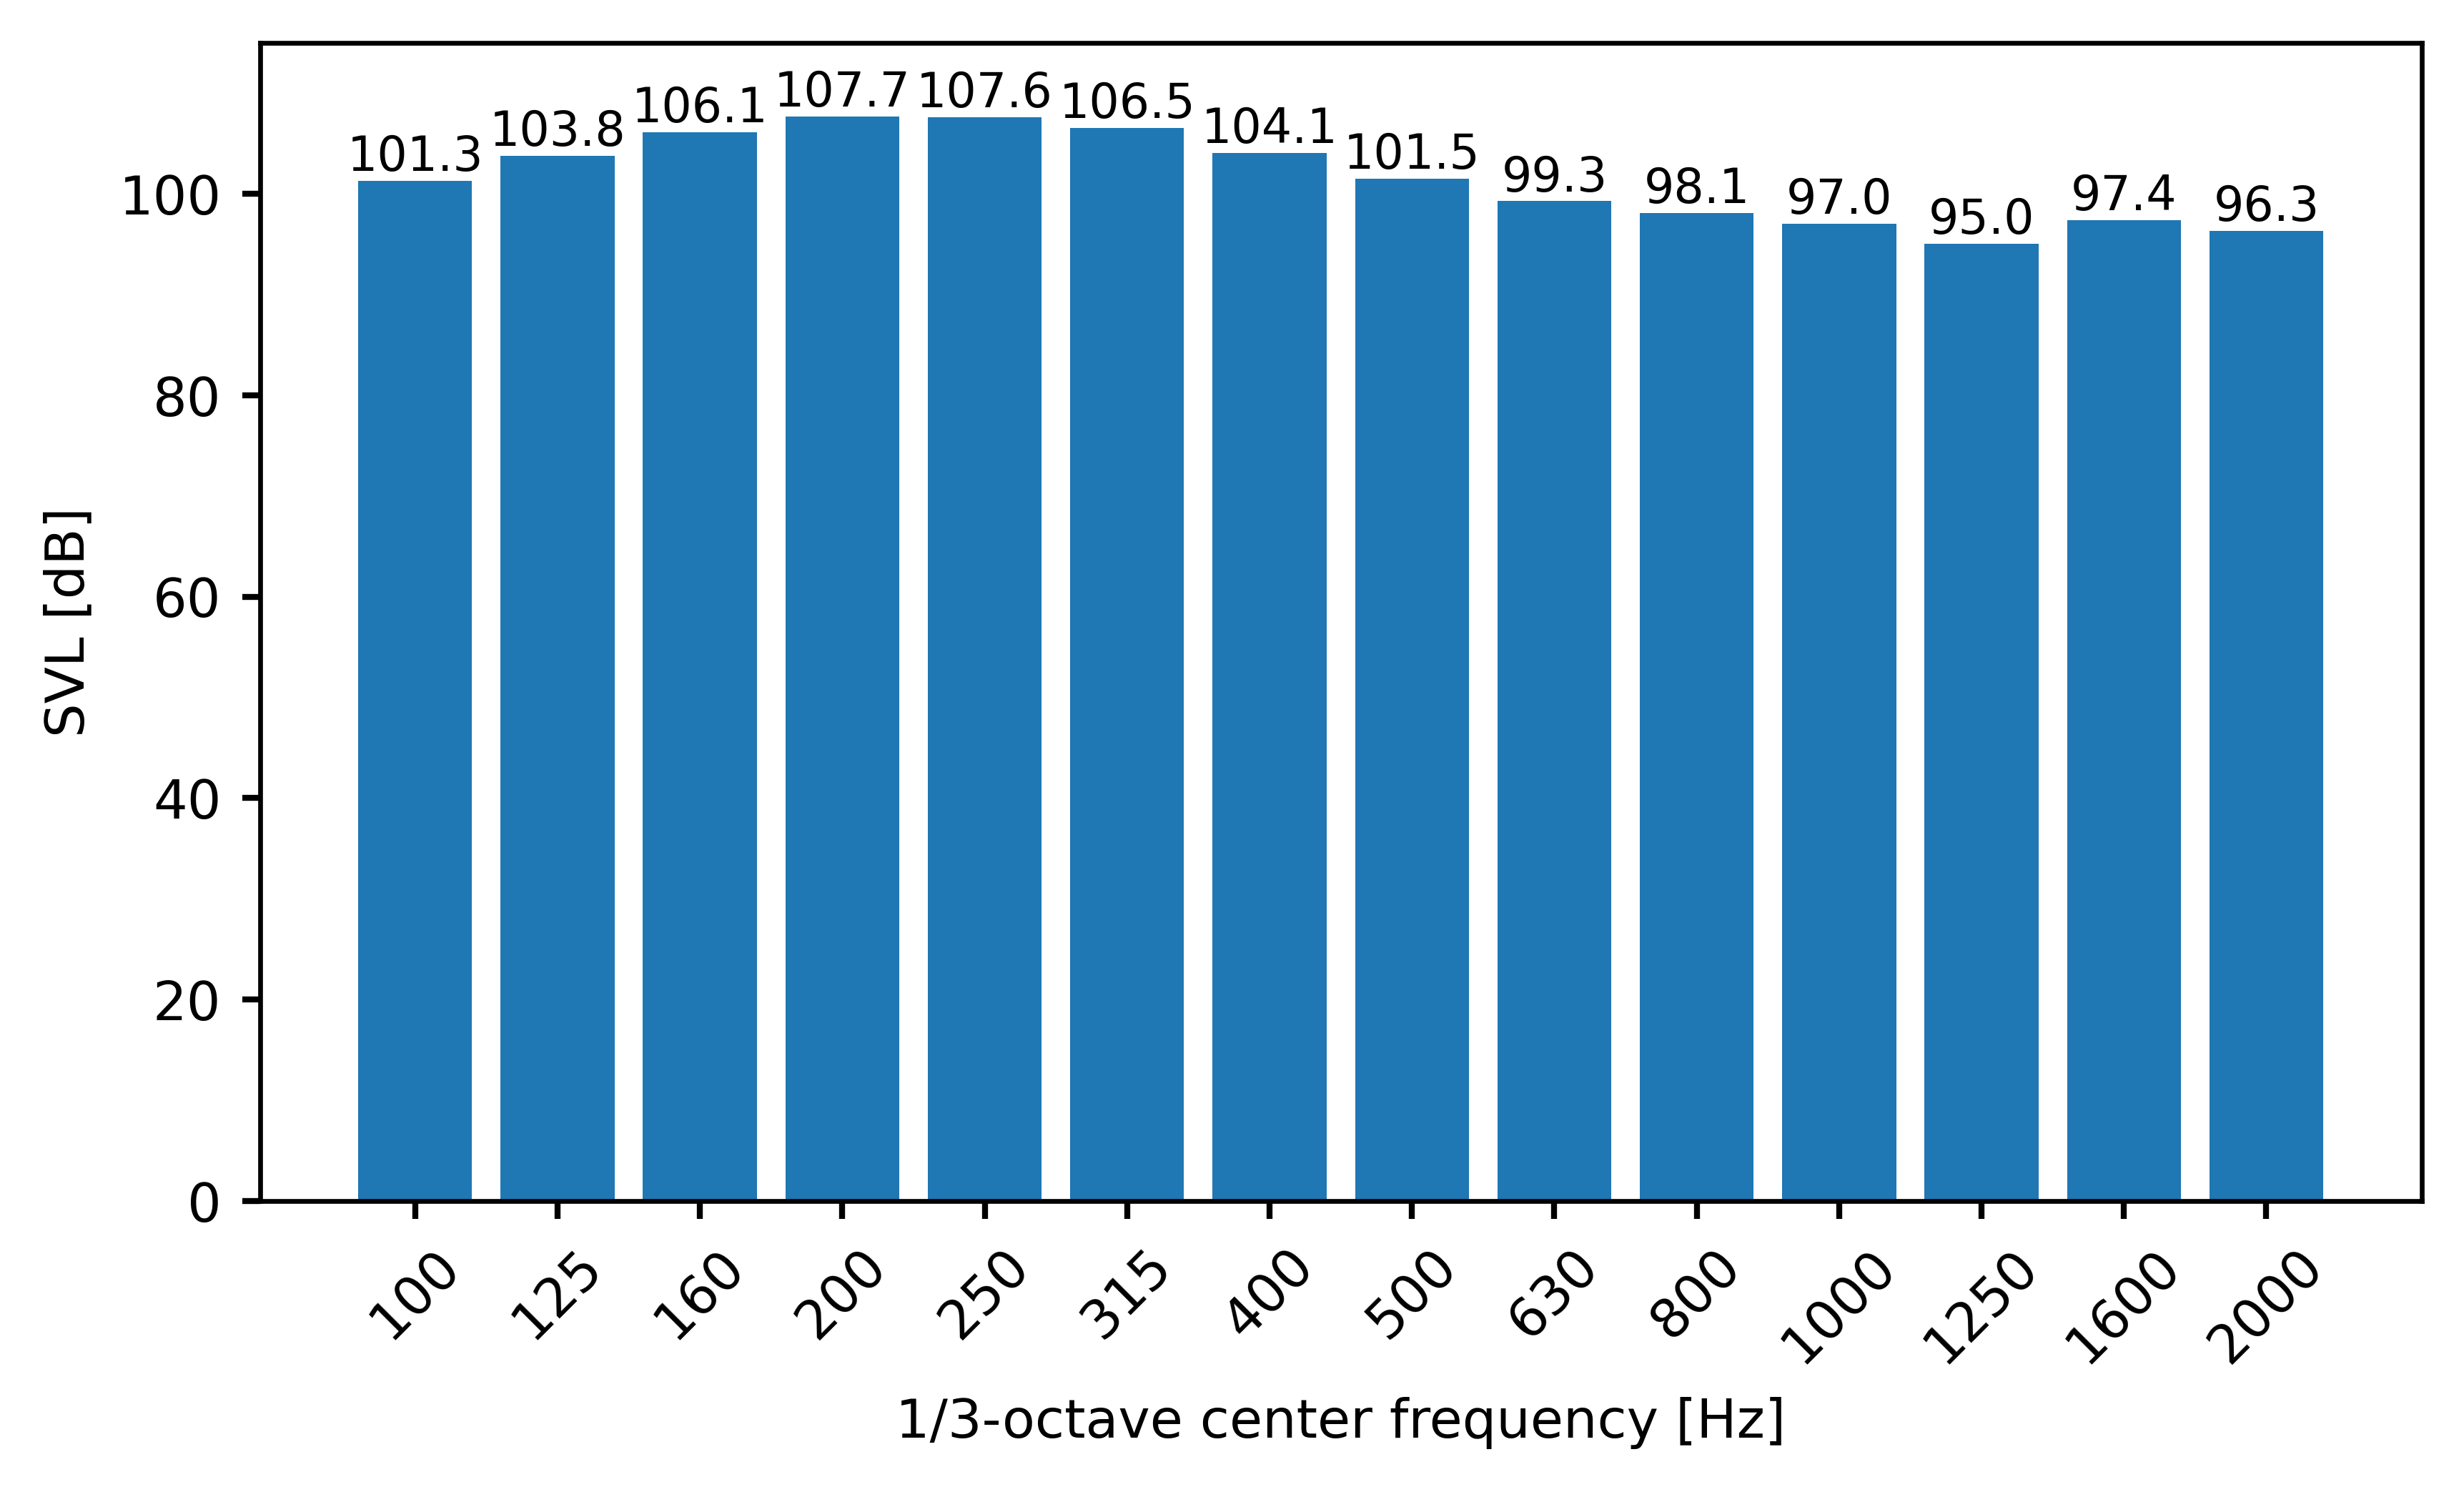
\includegraphics{fig/chap4/input_SVL.png}
	\caption{Input surface normal velocity in dB ref. $5\cdot10^{-8}\,\text{m/s}$, calculated using \ref{eq:input_velocity}}
\end{figure}

For the simulation, the sound power level of one single 1/3-octave band is divided into the 9 intermediate frequency steps by a 9.54 dB reduced sound power level for every single frequency within the band so that the sum of all frequencies results in the sound power level for the corresponding 1/3-octave band.




%\section{General simulation setup}
\newpage
\section{Parametric study}
\label{section:parametric_study}
\subsection{Variation of underfloor geometry}
\label{section:variation_geometry}

In the initial geometric setup, the contemplated underfloor components in the finite element model are the bogie frame, the wheel with axle, and the air suspension. In order to investigate the stability of simulation results to different underfloor geometrical setups, a parametric study with a variation of the underfloor geometry is carried out in the following.

\begin{figure}[H]
	\centering
	\begin{subfigure}[b]{0.49\textwidth}
		\centering
		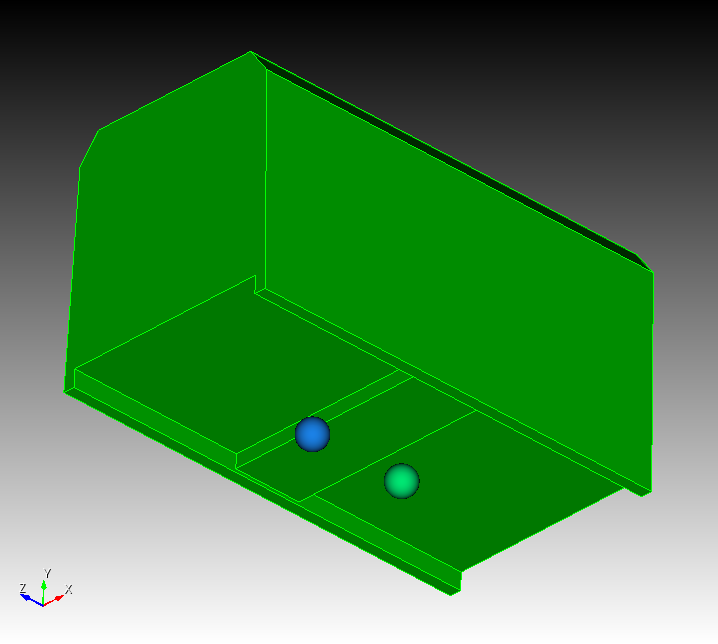
\includegraphics[width = 0.8\linewidth]{fig/chap4/geometry/no_underfloor_components_2.png}
		\caption{No underfloor components}
		\label{fig:no_underfloor_components}
	\end{subfigure}
	\begin{subfigure}[b]{0.49\textwidth}
		\centering
		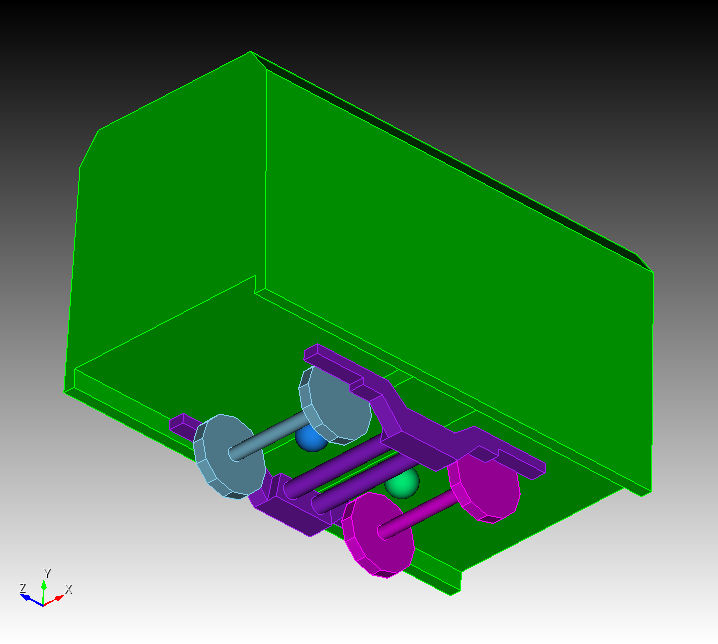
\includegraphics[width = 0.8\linewidth]{fig/chap4/geometry/no_air_suspension_2.png}
		\caption{No air suspension}
		\label{fig:no_air_suspension}
	\end{subfigure}
	\begin{subfigure}[b]{0.49\textwidth}
		\centering
		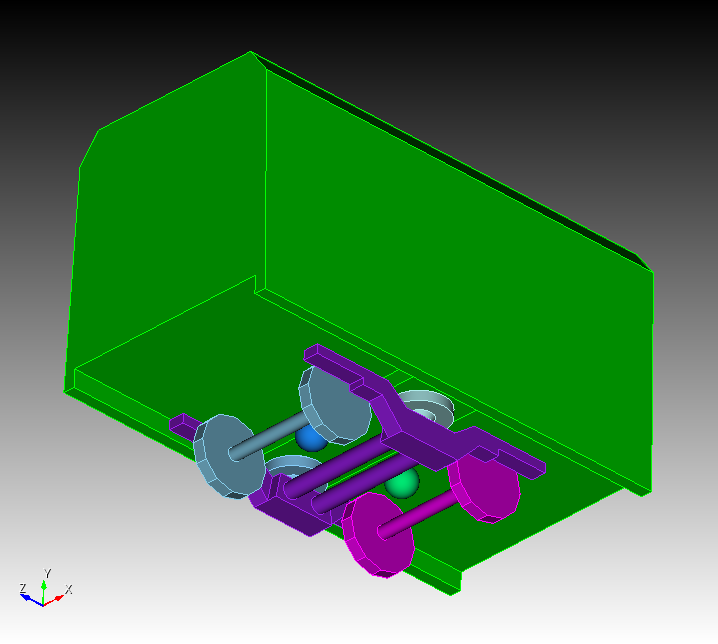
\includegraphics[width = 0.8\linewidth]{fig/chap4/geometry/initial_model_2.png}
		\caption{Initial model}
		\label{fig:initial_model}
	\end{subfigure}
	\begin{subfigure}[b]{0.49\textwidth}
		\centering
		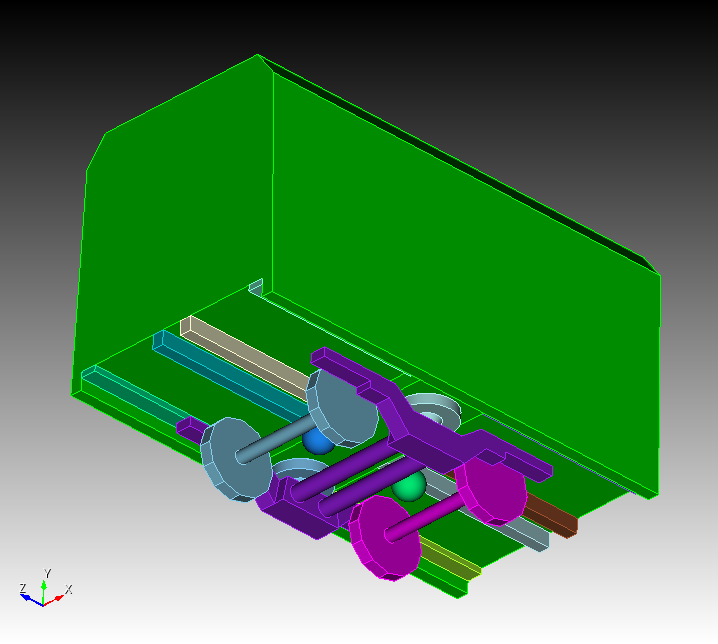
\includegraphics[width = 0.8\linewidth]{fig/chap4/geometry/additional_structures.png}
		\caption{Additional structures}
		\label{fig:additional_structures}
	\end{subfigure}
	\caption{Underfloor geometry with four variations.}
	\label{fig:variation_underfloor}
\end{figure}

For the parametric study, four different variations of underfloor geometry including the initial finite element model as described in \cref{section:geometry} are prepared, which are shown in \cref{fig:variation_underfloor}, ordered by their complexity. Again, the full model of each geometry is shown for a better illustration, whereby the one-fourth model will be used for the simulation. The simplest model (\cref{fig:no_underfloor_components}) contains only the car body shell without any underfloor components, the blue or the green sphere beneath the car floor represents the omnidirectional loudspeaker. In the next more complex model (\cref{fig:no_air_suspension}), the bogie frame and the wheels are contemplated, and differs from the initial geometry (\cref{fig:initial_model}) only by the air suspension, that is why this variation is also named "no air suspension". Finally, the last geometrical model (\cref{fig:additional_structures}) is set up by attaching additional structures to the car floor, which represent the cable ducts beneath the car floor.

\newpage
\subsection{Variation of ground surface impedance}

In the initial simulation setup, the ground is modeled as a fully reflective surface at which the homogeneous Neunmann (sound hard) boundary condition is applied.
However, it would also be of interest to investigate the influence of including ground absorption on the simulation result.
An absorbing surface is characterized by its absorption coefficient $\alpha$, which is frequency dependent in most cases.
In the finite element formulation, the reflection and absorption of the incident acoustic wave at a surface is described by the surface impedance boundary condition, which can be related to the absorption coefficient of the surface. In the following, the relation between the absorption coefficient $\alpha$ and the surface impedance $Z_s$ is presented following Nedkov \cite{nedkov_impedance_2011}.

The sound absorption coefficient $\alpha$ of a material is defined by the ratio of the absorbed acoustic power $W_{\text{absorbed}}$ and the power of incident wave $W_{\text{incident}}$, which for wave at normal incidence reads as
\begin{equation}
	\alpha = \frac{W_{\text{absorbed}}}{W_\text{incident}} = 1 - |R|^2\,, \label{eq:absorption_coefficient}
\end{equation}
with $R$ being the complex reflection coefficient, which can be represented as
\begin{equation}
	R = \frac{Z_s - Z_0}{Z_s + Z_0} = \frac{\frac{Z_s}{Z_0} - 1}{\frac{Z_s}{Z_0} + 1}\,, \label{eq:reflection_coefficient}
\end{equation}
where $Z_0 = \rho_0 c_0$ is the characteristic impedance of the propagation medium and $Z_s$ is the specific acoustic impedance of the absorbing surface.
The impedance ratio $\frac{Z_s}{Z_0}$ is also called the normalized surface impedance
\begin{equation}
	\tilde{Z_s} = \frac{Z_s}{Z_0} = \tilde{R_s} + j\tilde{X_s}\,,
\end{equation}
which can be slit into a real part $\tilde{R_s}$ and an imaginary part $\tilde{X_s}$. By inserting \cref{eq:reflection_coefficient} into \cref{eq:absorption_coefficient}, the absorption coefficient $\alpha$ can be related to the complex surface impedance by
\begin{equation}
	\alpha = \frac{4\tilde{R_s}}{\tilde{R_s}^2+\tilde{X_s}^2 + 2\tilde{R_s} + 1} \,. \label{eq:absorption_coefficient_2}
\end{equation}
In order to uniquely define the surface impedance $\tilde{Z_s}$ of the absorbing surface for a given normal incident absorption coefficient $\alpha$, the phase of the complex surface impedance also has to be known, which is given by
\begin{equation}
	 \varphi = \arctan{\frac{\tilde{X_s}}{\tilde{R_s}}}\,. \label{eq:impedance_phase_angle}
\end{equation}
The impedance characteristic of a ground surface can be determined for example by an in-situ measurement using impedance tube method \cite{wolkesson_2013,Seybert2008MeasurementOP}.
For the case that a measurement is not accessible, the absorption data can be retrieved e.g. from a acoustic data bank, which, in most cases, provides only the absorption coefficient spectrum in stead of the complex surface impedance.
However, it has been shown that also the phase has to be provided to uniquely define the surface impedance for a given absorption coefficient.
In order to have an idea how the missing information of the impedance phase angle affects the simulation result, surface impedance boundary condition is prescribed at the ground of the finite element model using varying impedance phase angle.

\begin{figure}[H]
	\centering
	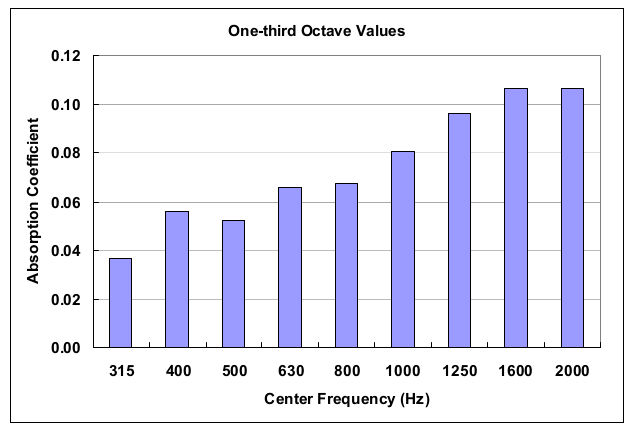
\includegraphics[width=0.7\textwidth]{fig/chap4/impedance/absorption_spectrum.png}
	\caption{Absorption coefficient in one-third octave bands \cite{Seybert2008MeasurementOP}}
	\label{fig:ground_absorption}
\end{figure}

Due to a missing ground absorption measurement, the absorption spectrum from the pavement absorption measurement carried out by Seybert et al. \cite{Seybert2008MeasurementOP} is used, which is shown in \cref{fig:ground_absorption}.
The values of the absorption coefficients are estimated from the graph and are listed in \cref{tab:absorption_coefficient} since these were not provided in the paper. For frequencies lower than \SI{315}{\hertz}, the absorption coefficient is set to 0.02. The complex normalized surface impedance can then be calculated by solving the system of equations consists of \cref{eq:absorption_coefficient_2} and \cref{eq:impedance_phase_angle}. Thereby, the impedance phase angle $\varphi$ is assumed to be \SI{0}{\degree} (only real part), $\pm$\SI{30}{\degree}, $\pm$\SI{45}{\degree}, and $\pm$\SI{60}{\degree}, respectively. The obtained normalized surface impedance spectra for different impedance phase angles are shown in \cref{fig:input_impedance}.

\begin{table}[H]
	\centering
	\caption{Estimated absorption coefficient from \cref{fig:ground_absorption}, for frequencies lower than 315 Hz the values are set to 0.02.}
	\label{tab:absorption_coefficient}
	\begin{tabular}{cccc}
		\toprule
		Frequency (Hz) & $\alpha$ & Frequency (Hz) & $\alpha$ \\
		\midrule
		100 & 0.02 & 500 & 0.05 \\
		125 & 0.02 & 630 & 0.065 \\
		160 & 0.02 & 800 & 0.065 \\
		200 & 0.02 & 1000 & 0.08 \\
		250 & 0.02 & 1250 & 0.095 \\
		315 & 0.035 & 1600 & 0.105 \\
		400 & 0.055 & 2000 & 0.105 \\
		\bottomrule
	\end{tabular}
\end{table}

\begin{figure}[H]
	\centering
	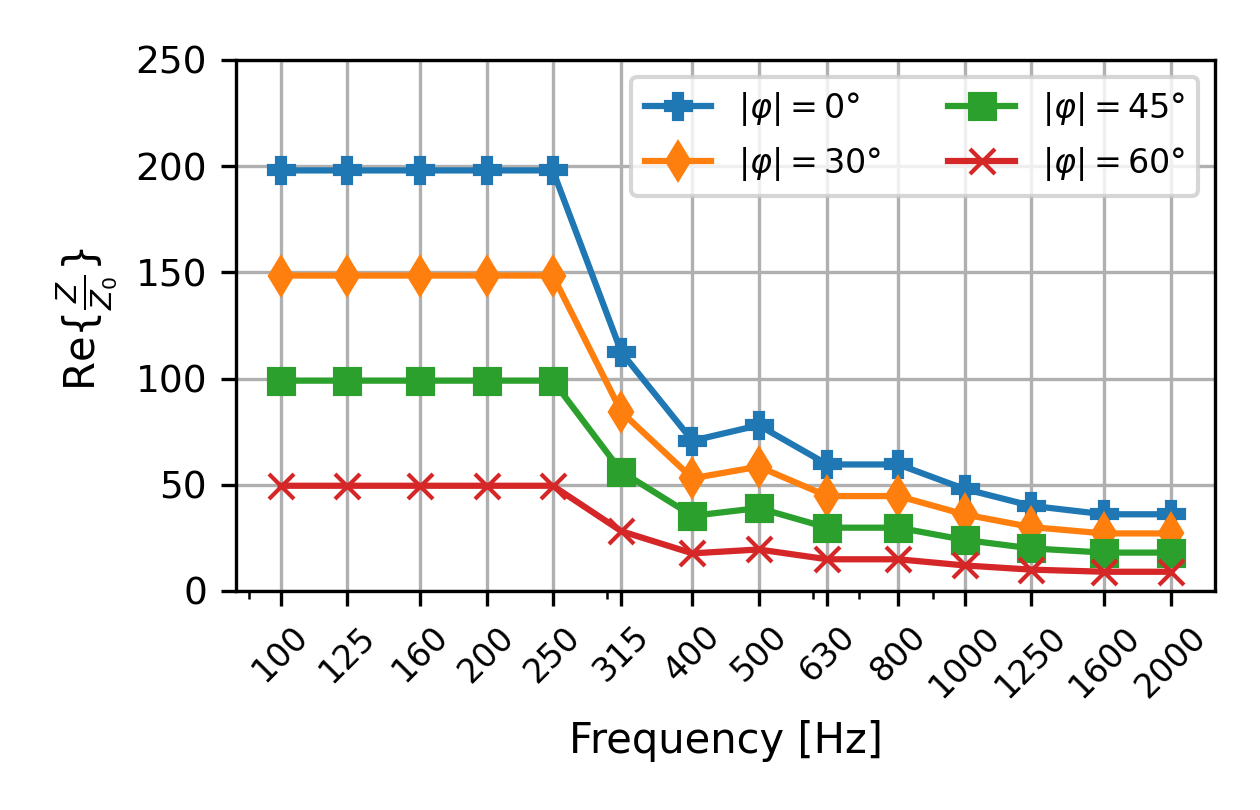
\includegraphics{fig/chap4/impedance/impedance_real.png}
	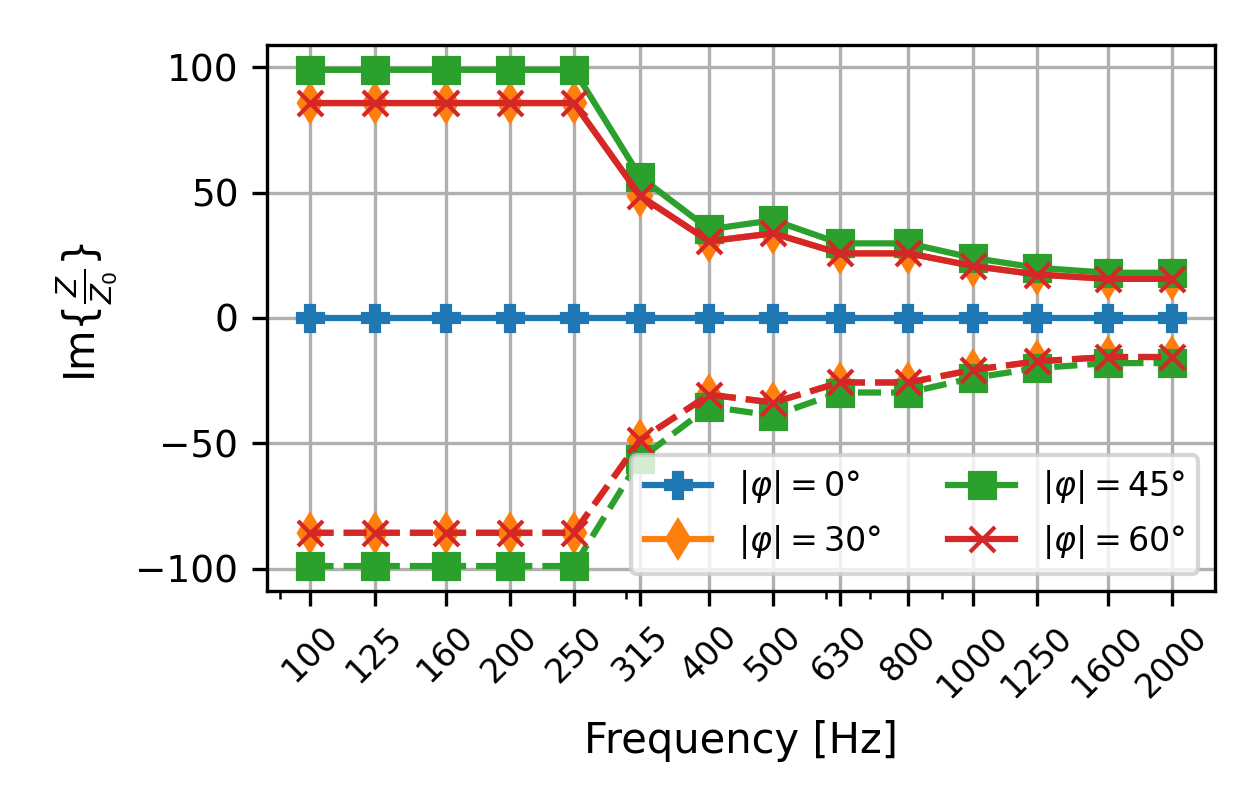
\includegraphics{fig/chap4/impedance/impedance_imag.png}
	\caption{Real and imaginary part of the surface impedance normalized by $Z_0 = \rho_0 c_0$ calculated by solving \cref{eq:absorption_coefficient_2} and \cref{eq:impedance_phase_angle}.}
	\label{fig:input_impedance}
\end{figure}

\newpage
\subsection{Variation of frequency steps per 1/3-octave band}

In this thesis, the simulation and the measurement results will be compared in one-third octave bands.
In the initial simulation setup, each one-third octave band is computed using nine intermediate frequency steps corresponding to the 1/24-octave center frequencies to ensure a sufficient frequency band resolution.
However, the computation time of single one-third octave band grows almost linearly with the number of intermediate frequency steps.
As already shown in \cref{section:geometry}, the computation time of the highest frequency band \SI{2000}{Hz} using nine intermediate frequencies almost takes up half of the total simulation run time.
Therefore, it would be of great interest to find a proper number of intermediate frequency steps per one-third octave band, which can lower the computational effort of the simulation while providing a similar numerical accuracy.

For the parametric study, each one-third octave band is computed using one, three, five, and nine intermediate frequency steps, respectively. Obviously, there are several possibilities for choosing the frequencies used within the octave band. However, this study concentrates on the influence of the number of frequencies used on the simulation results but not the different selection of the frequencies. Therefore, a rule for choosing the frequencies used within the one-third octave band will be defined for each number of steps. For the single frequency step, the center frequency of the corresponding one-third octave band is used. Next, for the model using three intermediate steps, the lower and the upper frequency limits of the one-third octave band are additionally used, corresponding to the 1/6-octave center frequencies. Finally, the frequencies used for five steps and nine steps are equivalent to the 1/12-octave center frequencies and the 1/24-octave center frequencies within the one-third octave frequency band, respectively. An example of the frequency selection for \SI{1000}{\hertz} one-third octave band is shown in \cref{tab:variation_freq_steps}. The same selection criteria apply to other one-third octave bands.

\begin{table}[H]
	\caption{Choice of frequencies used for different number of intermediate steps, example one-third octave band \SI{1000}{\hertz}.}
	\centering
	\begin{tabular}{ccc}
		\toprule
		Number of steps    &  Frequencies used (Hz) & Note  \\
		\midrule
		1    &  1000  & 1/3-octave center frequency\\
		3  	 &  891, 1000, 1122 & 1/6-octave center frequencies \\
		5  	 &  891, 944, 1000, 1059, 1122 & 1/12-octave center frequencies\\
		9    &  891, 917, 944, 972, 1000, 1029, 1059, 1091, 1122 & 1/24-octave center frequencies \\
		\bottomrule
	\end{tabular}
	\label{tab:variation_freq_steps}
\end{table}